\documentclass{mwhittaker}
\title{Deep RL Assignment 4}
\date{October 18, 2017}

\usepackage{graphicx}

\newcommand{\tabref}[1]{Table~\ref{tab:#1}}
\newcommand{\figref}[1]{Figure~\ref{fig:#1}}

\begin{document}
\maketitle
\tabref{data} shows the average, standard deviation, min, and max cost and
return over all 15 iterations of training. The first row corresponds to a model
trained on random data alone. We see an average return of 231. \figref{data}
plots the average return over all 15 iterations. Wee see that on-policy data
greatly improves the model. After one iteration of training with on-policy
data, the average return nearly quadruples.

\begin{table}[ht]
  \footnotesize
  \begin{tabular}{|l|l|l|l|l|l|l|l|l|l|}
    \hline
    Iteration & AvgCost  & StdCost & MinCost  & MaxCost  & AvgReturn & StdReturn & MinReturn & MaxReturn \\\hline
    0         & -305.27  & 25.67   & -335.48  & -260.24  & 231.85    & 21.17     & 196.29    & 260.65\\\hline
    1         & -1089.21 & 45.63   & -1149.30 & -1020.15 & 929.65    & 45.31     & 859.67    & 986.29\\\hline
    2         & -1249.70 & 39.67   & -1306.63 & -1182.14 & 1077.23   & 37.34     & 1020.26   & 1129.01\\\hline
    3         & -1409.24 & 80.72   & -1529.62 & -1254.19 & 1255.22   & 77.12     & 1083.74   & 1342.68\\\hline
    4         & -1401.79 & 43.71   & -1456.18 & -1318.92 & 1254.14   & 39.16     & 1181.10   & 1315.06\\\hline
    5         & -1367.99 & 41.39   & -1463.23 & -1312.81 & 1182.44   & 33.12     & 1145.12   & 1264.08\\\hline
    6         & -1490.21 & 46.05   & -1585.24 & -1431.01 & 1307.46   & 47.82     & 1241.20   & 1421.24\\\hline
    7         & -1553.30 & 78.60   & -1666.55 & -1425.96 & 1375.82   & 75.81     & 1250.11   & 1482.06\\\hline
    8         & -1519.92 & 58.90   & -1635.27 & -1457.52 & 1325.36   & 57.85     & 1260.00   & 1449.40\\\hline
    9         & -1574.72 & 42.86   & -1651.14 & -1507.69 & 1402.48   & 47.08     & 1324.96   & 1502.44\\\hline
    10        & -1574.72 & 57.17   & -1665.89 & -1488.55 & 1391.79   & 50.25     & 1315.75   & 1476.28\\\hline
    11        & -1534.18 & 60.76   & -1622.66 & -1436.99 & 1357.33   & 63.13     & 1228.05   & 1438.34\\\hline
    12        & -1539.63 & 68.40   & -1607.17 & -1379.15 & 1367.83   & 64.62     & 1215.96   & 1461.46\\\hline
    13        & -1536.60 & 80.15   & -1681.37 & -1412.66 & 1355.68   & 76.55     & 1225.67   & 1488.31\\\hline
    14        & -1582.14 & 68.34   & -1681.52 & -1440.53 & 1391.32   & 71.55     & 1231.38   & 1487.24\\\hline
  \end{tabular}
  \caption{Log output for every iteration.}
  \label{tab:data}
\end{table}

\begin{figure}[ht]
  \centering
  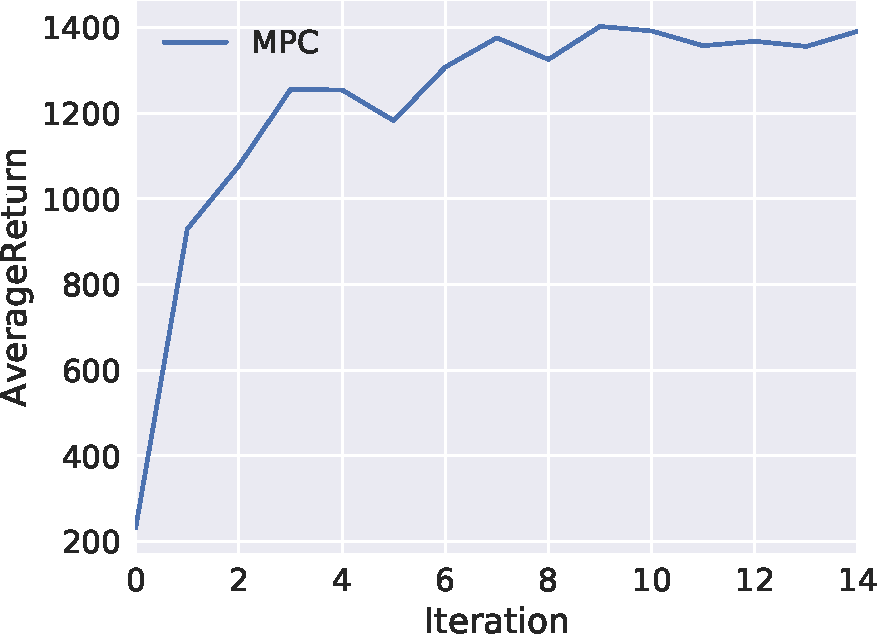
\includegraphics[width=0.6\textwidth]{returns.pdf}
  \caption{Average return over 15 iterations}
  \label{fig:data}
\end{figure}

\end{document}
